% Response to Editor
\editor

% todo ? 放原文吗

\begin{metacomment}
	Clearly differentiate the contributions from prior works.
\end{metacomment}
\begin{metaresponse}
\end{metaresponse}
	We appreciate your handling of the review process and highlighting this issue.
	Compared with previous works, our current further considers the complex overlapping or containing range relationship between sensors.
	We have revised Section 1 to better highlight the challenge introduced by this relationship and to underscore their practical relevance in real-world scenarios.
	
	The revised description of this relationship and the associated challenge are given below, respectively.
	\begin{changes}
		This altitude-dependent coverage creates intricate spatial relationships between sensors, manifesting in various overlapping patterns: partial overlap, full containment, reverse containment, and disjointness.
		Moreover, these relationships become even more complex as communication range changes with altitude, creating challenges that have not been fully addressed in previous research.
		For example, in Fig.~1, as the altitude increases, sensor $S_1$ initially overlaps with $S_2$, but eventually becomes fully contained by $S_2$.
		Such overlapping range relationship better captures the complexity of real-world scenarios and provides practical value for UAV-assisted data collection.
		Capturing and fully exploiting these altitude-dependent ranges is crucial, since it enables the data from a single sensor to be collected across multiple sessions and fundamentally influences the order of data collection.
	\end{changes}
	\begin{changes}
		Due to the complex overlapping patterns of sensor data transmission ranges, the UAV is often simultaneously located within the ranges of multiple sensors. Consequently, determining the optimal data collection sequence becomes highly challenging.
	\end{changes}
\begin{metacomment}
	Address limitations for practical application of the algorithm.
\end{metacomment}
\begin{metaresponse}
	We appreciate your careful review and comment.
	The reviewers pointed out the practical limitations of our work, including the assumptions of linear ground node (GN) deployment and complete GN knowledge, as well as the applicability of the proposed algorithm to 3D GN layouts.
	We have discussed these assumptions and provided a strategy to address 3D GN layout scenarios.
	% 几个假设
	% vertical energy consumption
	% 3D GN layout
	% linear deployment
	% complete GN knowledge -> Probe-ACK的过程
	% real-world path loss effects

	\textbf{Linear GN deployment.}
	The linear configuration of GNs represents a reasonable and commonly utilized setup in real-world systems.
	This deployment pattern often arises in infrastructure monitoring scenarios.
	For instance, in the power line~\cite{powerline,transmission-line}, UAVs are dispatched to autonomously collect data from sensors on the transmission tower.
	Similarly, in the oil and gas industry~\cite{pipeline}, UAVs are used to fly along pipelines for inspection activities.
	In addition, sensors can be deployed along rivers~\cite{river} and coasts~\cite{coast} to capture diel and seasonal fluctuations, with the purposes of ecological monitoring, flood warning, and scientific research.

	In fact, the effectiveness of such linear GN deployment has already been demonstrated in industrial applications to reduce costs, improve work efficiency, and avoid hazardous manual tasks.
	For instance, DJI has successfully implemented UAV-enabled solutions in scenarios such as long-distance pipelines~\cite{DJI-pipeline}, power transmission line in plateau regions~\cite{DJI-powerline}, and river ecosystems~\cite{DJI-river}, where the UAV trajectories can be regarded as linear or the combination of multiple straight-line segments.

	\textbf{GN knowledge.}
	Sensor knowledge mainly includes information such as position, amount of data to be collected, transmission rate, and data transmission range.
	(1) In the online problem, each sensor has an additional control communication range, which covers a larger area than the data transmission range.
	When the UAV enters the sensor's control communication range, it can detect the sensor and receives a response containing information such as the amount of data and the sensor's position.
	We have explained this process in the revised manuscript as shown below.
	(2) There is a proportional relationship between the radius of the data transmission range and the control communication range.
	Based on the distance between the sensor and the UAV at the moment the response is received, the radius of the data transmission range can be estimated.
	(3) The sensor position is fixed, and thus, it can be obtained during the initial deployment and periodic maintenance. This allows for the calibration of sensor positions.
	\begin{changes}
		The UAV keeps broadcasting `Probe' message during the flight to detect sensors. Once receiving the `Probe' message, the sensor sends back an `ACK' message, which includes its position, the amount of data, and transmission characteristics. Note that each sensor sends `ACK' message only once. This partial information availability fundamentally changes the nature of our optimization problem, requiring real-time 
		decision-making based on local information.
	\end{changes}

	\textbf{3D GN layout.}
	% Our current focuses on the linear (2D) GN distribution, including power transmission lines, roads, pipelines, river and coast.
	By integrating advanced trajectory planning methods, our algorithms can be extended to 3D GN layout.
	% 
	Specifically, we first apply a trajectory planning algorithm to optimize the UAV's flight path and avoid collisions.
	The area of UAV trajectory planning and collision avoidance has been extensively studied in recent years.
	The distance travelled from the starting point to any location along the trajectory is treated as the horizontal coordinate of that location.
	Along this trajectory, we can then use SSF-ACO algorithm to jointly optimize speed and altitude scheduling.
	
	Although promising, this approach to extending the 3D GN layout remains subject to certain limitations.
	Jointly optimizing the 3D trajectory and speed scheduling is expected to have a better performance.
	Furthermore, the increased computational complexity associated with 3D scheduling problems presents additional challenges.
	However, these issue fall within a broader area that extends beyond the focus of the current work.
	Addressing them remains also one of our future research directions.
	In this work we concentrate on the optimization of speed and altitude scheduling, and demonstrate compatibility with existing trajectory planning algorithms.
\end{metaresponse}

\begin{metacomment}
	Validate the claim of ``near-optimal performance.''
\end{metacomment}
\begin{metaresponse}
	Thank you for highlighting this issue.
	We recognize that the term ``near-optimal'' was not precise. Our intention was to indicate that SSF-ACO-Online performs closely to the offline algorithm SSF-ACO. We have revised the abstract to clarify this point and removed the term ``near-optimal'' to avoid confusion.
	\begin{changes}
		Extensive simulations demonstrate that SSF-ACO significantly outperforms baseline approaches in energy efficiency, and SSF-ACO-Online achieves comparable performance with energy consumption 1.24\% higher than offline counterpart in average.
	\end{changes}
\end{metaresponse}

\begin{metacomment}
	Test SSF-ACO and SSF-ACO-Online under network dynamics (e.g., node mobility).
\end{metacomment}
\begin{metaresponse}
	We appreciate the comment, which highlights important aspects that could influence the effectiveness the UAV scheduling.
	In the following, we will discuss the ground nodes (GNs) mobility, inaccurate position, failures, and unstable communication environment.

	\textbf{GN mobility.}
	GN mobility is an important factor in various UAV-assisted systems.
	However, our current work focuses on data collection from stationary sensors.
	In the scenarios we consider, the sensors are fixed in the environment to monitor infrastructures or natural conditions.
	Admittedly, a number of existing studies~\cite{GNmob1, GNmob2, GNmob3, GNmob4} have investigated GN mobility.
	In these studies, GNs typically refer to mobile user devices with significant movement, such as user-carried devices~\cite{GNmob1,GNmob2} or vehicles~\cite{GNmob3,GNmob4}, which are fundamentally different from the stationary GNs considered in our work.

	\textbf{Inaccurate position.}
	The proposed algorithm relies on the precise sensor positions.
	However, the inaccurate sensor localization leads to discrepancies between the UAV scheduling and actual environment.
	In our future, we intend to employ more advanced relative positioning techniques to reduce localization inaccuracy and incorporate error-tolerant strategies to improve the system's robustness and reliability.

	\textbf{Failures.}
	Failures may occur either before or during data transmission.
	Failures before transmission will result in the sensor being undetectable by the UAV.
	On the other hand, failures during the transmission process will lead to a disruption in the connection between the UAV and the sensor.
	The UAV will attemp to reconnect and, after reaching the maximum number of reconnection attempts, will abandon the connection.
	Regardless of whether reconnection is successful, the scheduling will be re-planned to ensure energy efficiency.

	\textbf{Unstable communication environment.}
	The changes in the communication environment may lead to fluctuations in the transmission rate.
	When the UAV first detects the sensor, it will receive the sensor's guaranteed minimum transmission rate included the sensor's `ACK' message.
	When the guaranteed minimum transmission rate is not met, the UAV's speed and altitude scheduling will be re-planned by our algorithm to adapt to the environment changes.
	In our work, variations in the communication environment are represented by different transmission rates, which in turn affect the required transmission duration. Accordingly, we evaluate the algorithms' performance under different required times.
	% todo 放实验图吗 
	% The results are shown in Figure~\ref{meta:fig:time}.

	% \begin{figure}[h]
	% 	\centerline{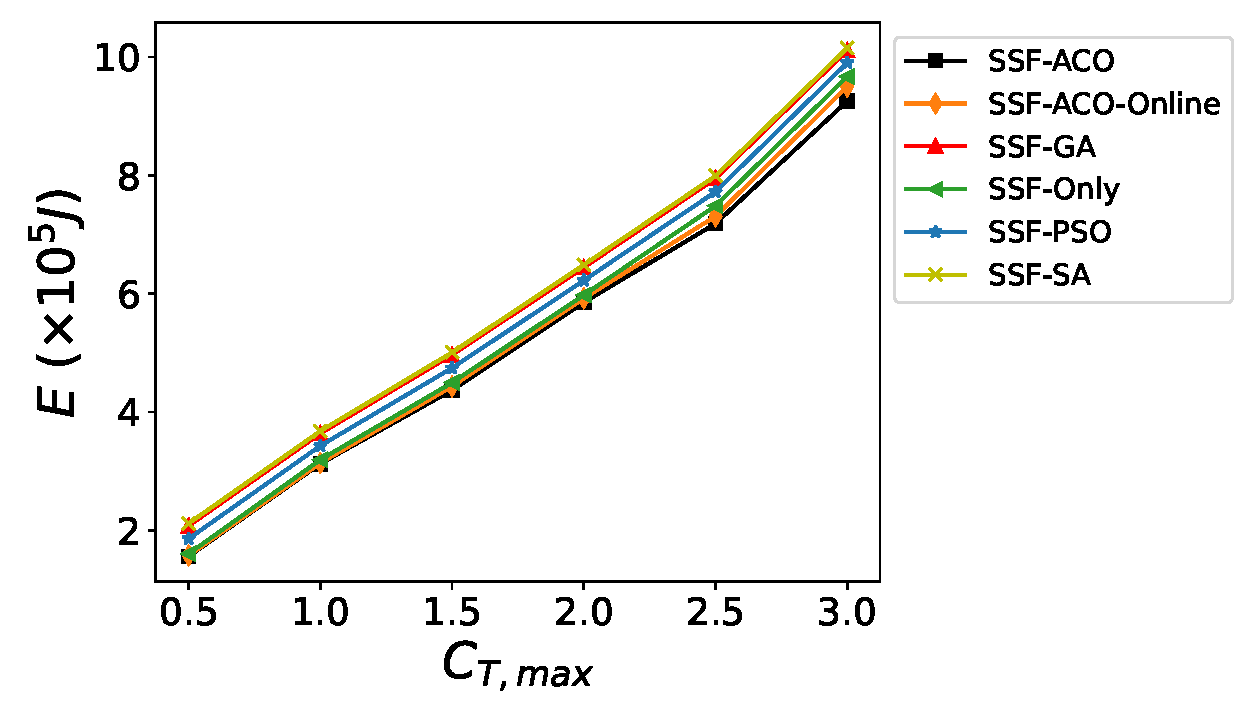
\includegraphics[width=.65\textwidth]{fig/exp_time_legend.pdf}}
	% 	\caption{Algorithm performance comparisons in UAV energy consumption under varying upper bound of data collection time coefficient.}
	% 	\label{meta:fig:time}
	% \end{figure}
\end{metaresponse}

\begin{metacomment}
	Explain the rationale behind heuristic factor selection.
\end{metacomment}
\begin{metaresponse}
	Thank you for the suggestion.
	In the algorithm, $\alpha$ and $\beta$ are the exponential parameters to control the influence of pheromone and heuristic values, respectively.
	We performed a grid-search over representative combinations of the pheromone exponential factor $\alpha\in\{1,2,3,4\}$ and heuristic exponential factor $\beta\in\{0,1,2,3,4\}$ to access parameter sensitivity as shown in Figure~\ref{meta:fig:cali}.
	The algorithm's performance under $\beta=0$ is significantly worse than performance for other parameter combinations. $\beta=0$ eliminates the use of heuristic information, resulting in purely random exploration during the initial iterations and thus poor performance.
	The results also indicate that the configuration $\alpha=1,\beta=2$ consistently achieves the minimum energy consumption. Accordingly, we adopted $\alpha=1,\beta=2$ in all simulation experiments.
	\begin{figure}[h]
		\centerline{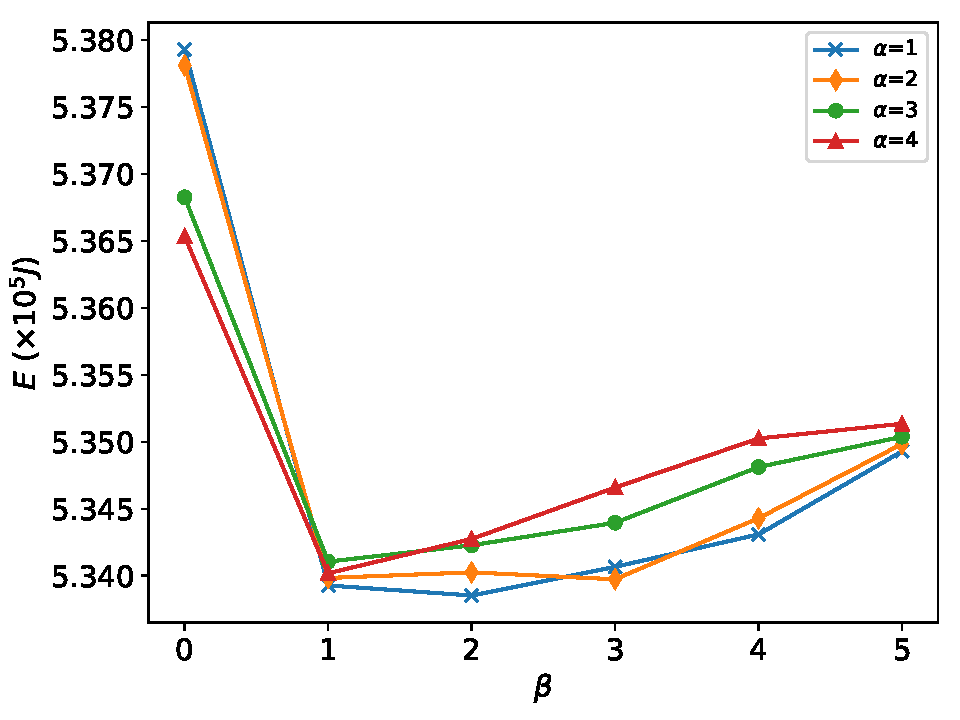
\includegraphics[width=.5\textwidth]{fig/cali.pdf}}
		\caption{Performance of SSF-ACO across different $(\alpha,\beta)$ combinations.}
		\label{meta:fig:cali}
	\end{figure}
\end{metaresponse}

\begin{metacomment}
	Include more comprehensive experimental validation.
\end{metacomment}
\begin{metaresponse}
	Thank you for the suggestion.
	We have extended the experiments to include scenarios with more sensors and analyzed the computational latency of SSF-ACO-Online to demonstrate its suitability for online scheduling.

	\textbf{Scalability to larger-scale problems.}
	Our algorithms are designed with scalability and is capable of handling larger-scale problems.
	To further verify its scalability, we extended the evaluation to include scenarios involving more ground sensor nodes. The updated results are illustrated in Figure~\ref{meta:fig:40nodes}, which is identical to Figure~8a in the manuscript. The results demonstrate that the proposed algorithms continue to exhibit superior performance even in larger-scale scenarios.

	\textbf{The computational latency of SSF-ACO-Online.}
	We have reported the cumulative computational time of SSF-ACO-Online and the corresponding UAV flight durations.
	These results are summarized in Table~\ref{meta:tb:runtime} (Table 4 in the manuscript) and discussed in the revised manuscript as follows to demonstrate the suitability of SSF-ACO-Online.

	\begin{changes}
		Finally, we analyze the computational latency of SSF-ACO-Online.
		Table~4 reports the duration of UAV flights $T_f$ under online problem, along with the computation time of SSF-ACO-Online $T_{on}$, and that of SSF-ACO $T_{off}$ in the corresponding offline problem.
		Across varying numbers of sensors, the computation times of SSF-ACO-Online stay under 6 seconds and constitute no more than 0.19\% of the corresponding UAV flight duration.
		This demonstrates the suitability of SSF-ACO-Online for online applications.
		Since the active sensor list only maintains those sensors that have been discovered but not yet completely collected, though invoked SSF-ACO multiple times, SSF-ACO-Online has a cumulative computation time significantly shorter than that of SSF-ACO.
	\end{changes}

	\begin{figure}[h]
		\centerline{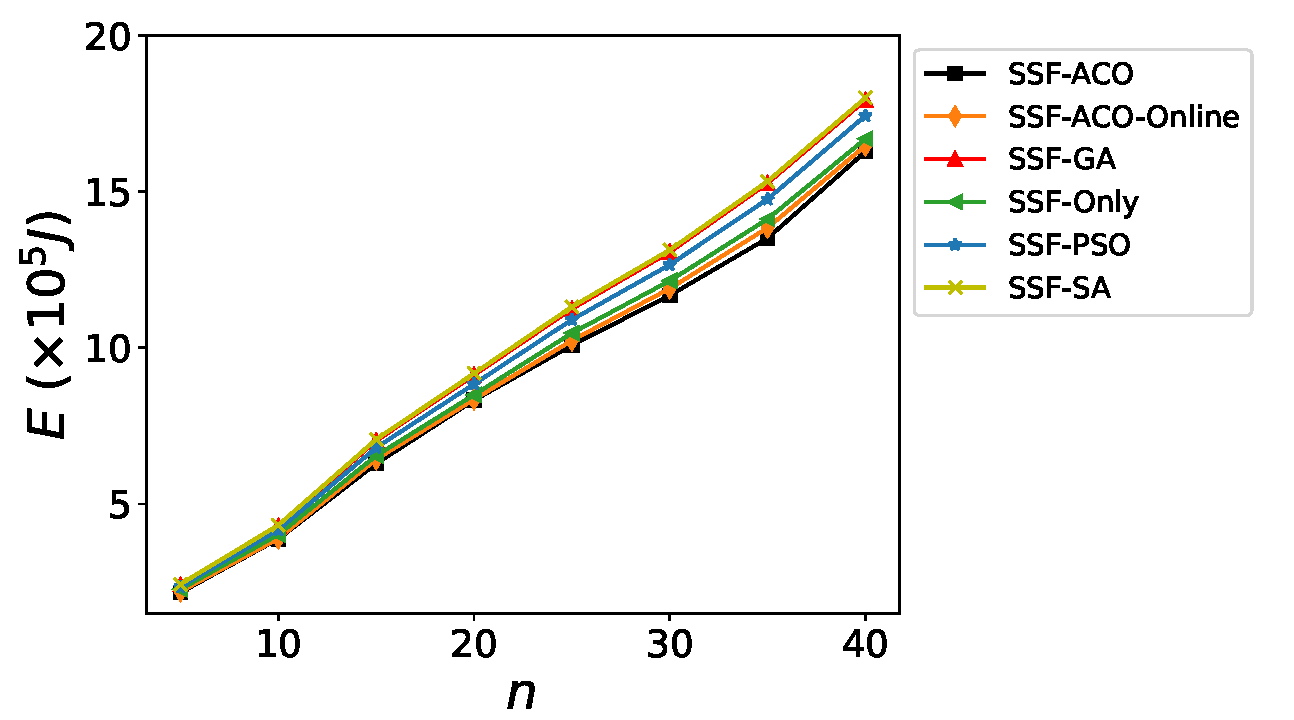
\includegraphics[width=.65\textwidth]{fig/exp_number_40_legend.pdf}}
		\caption{Algorithm performance comparisons in UAV energy consumption under varying numbers of sensors.}
		\label{meta:fig:40nodes}
	\end{figure}

	\begin{table}[h]
		\renewcommand{\arraystretch}{1.2}
		\centering
		\caption{Computation Time of SSF-ACO and SSF-ACO-Online Compared with UAV Flight Duration in Online Scheduling (in Seconds)}
		\label{meta:tb:runtime}
		\centering
		\begin{tabular}{*{9}{c}}
			\hline
			$n$ & 5 & 10 & 15 & 20 & 25 & 30 & 35 & 40 \\
			\hline
			$T_f$ & 513.73 & 1107.11 & 1502.68 & 2084.67 & 2675.47 & 2997.83 & 3519.72 & 4119.79 \\
			$T_{off}$ & 1.58 & 5.60 & 12.01 & 19.11 & 32.32 & 51.01 & 64.60 & 92.73 \\
			$T_{on}$ & 0.99 & 1.81 & 2.91 & 3.09 & 3.49 & 3.87 & 5.04 & 5.80 \\
			$T_{on} / T_f$ & 0.19\% & 0.16\% & 0.19\% & 0.15\% & 0.13\% & 0.13\% & 0.14\% & 0.14\% \\
			\hline
		\end{tabular}
	\end{table}

\end{metaresponse}

\begin{metacomment}
	Extend the discussion of related literature for completeness.
\end{metacomment}
\begin{metaresponse}
	Thank you for highlighting this issue.
	We have extended the discussion of related literature in the revised manuscript, especially in Section 2.3 regarding optimization algorithms for UAV-assisted systems.
	Popular algorithms are divided into three categories, including mathematical optimization techniques, heuristic algorithms, and learning-based methods. Their limitations are discussed.
	The revised Section 2.3 is as follows:
	\begin{changes}
		The optimization of UAV-assisted systems has attracted significant research attention, with various algorithms proposed to minimize energy consumption. 
		These approaches can be classified into three main categories.

		Mathematical optimization techniques were applied when the problem structure allowed theoretical analysis. 
		For instance, Shan \etal~\cite{SLXWL-INFOCOM20} derived optimal policies for linear data collection by constructing temporal-spatial constraints. 
		Other works~\cite{b-math1,b-math2} employed successive convex approximation for non-convex problems. 
		However, these methods often imposed strict assumptions on problem formulation and could be computationally intensive.

		Learning-based methods, particularly deep learning (DL) and RL, gained popularity in recent years, as they learned complex parameters or action policies during the training process.
		In UAV-assisted mobile edge computing systems, Lin \etal~\cite{b-DL} proposed a parametrized dueling deep Q-network to maximize the UAV's energy efficiency.
		The problem was formulated as a mixed-integer nonlinear programming (MINLP) problem, which facilitated the modeling of problems involving both continuous variables (\eg trajectory) and discrete variables (\eg data collection decision and task offloading decision).
		To maximize the total throughput and energy efficiency, Chen \etal~\cite{b-RL} formulated long-term UAV-aided data collection problem as a Markov Decision Process (MDP), and addressed it by a multi-agent DRL algorithm.
		However, the maximum number of ground nodes that could be served in \cite{b-DL} and \cite{b-RL} was only 6 and 8, respectively, as the extremely high computational complexity became unacceptable when the number of ground nodes increased.
		Hao \etal~\cite{hao-minlp} formulated a task offloading problem in a UAV-assisted mobile edge computing system as a MINLP, and then transformed it into a MDP.
		The problem was solved by a DRL algorithm.
		Zhong \etal~\cite{zhong-minlp} also applied a similar approach to address a task offloading and resource allocation problem.
		Despite their successful application to larger-scale problems, challenges still remain in the context of the JUSAS problem, particularly in modeling the environment and designing the reward function, including aligning the reward signal with the objective and dealing with sparse rewards.

		Heuristic algorithms were widely applied due to their greater flexibility and practical applicability.
		Fu \etal~\cite{a-heuristic1} considered a mobile crowdsensing scenario where UAVs collected data from mobile devices, and proposed a lightweight heuristic navigation algorithm to optimize UAVs' trajectory.
		The authors employed multiple virtual search agents to iteratively seek a satisfactory destination.
		Similarly, Lin \etal~\cite{a-heuristic3} developed a heuristic hexagon-based scheduling algorithm to improve eneryg efficiency for periodic data collection using UAVs,
		and also proposed an emergent node charging scheduling method to prevent node exhaustion.
		To reduce cost, Gong \etal~\cite{a-heuristic2} incorporate particle swarm optimization (PSO) algorithm to minimize the number of UAVs required to visit all sensors.
		Other meta heuristic algorithms included genetic-based algorithms~\cite{a-heuristic4} and simulated annealing (SA) algorithm~\cite{liao2024energy}.
		However, these methods are not readily applicable to the JUSAS problem.
	\end{changes}
\end{metaresponse}

% todo ? 需要吗
\printpartbibliography{powerline,transmission-line,pipeline,river,coast,DJI-pipeline,DJI-powerline,DJI-river,SLXWL-INFOCOM20,b-math1,b-math2,b-DL,b-RL,hao-minlp,zhong-minlp,a-heuristic1,a-heuristic2,a-heuristic3,a-heuristic4,liao2024energy}
